%%%%%%%%%%%%%%%%%
% \chapter{}
% \section{}
% \subsection{}
% \subsubsection{}
% 
% \includegraphics[width=0.8\textwidth]{}
%
% \begin{itemize} 
%		\item 
% \end{itemize}
%
%
%	\npar
% \begin{quote}
%		\textbf{titel van de tabel}
%		\npar
%		\begin{tabular}{|cc|c|r|r|}
%			\hline
%				\multicolumn{2}{|c|}{Topleft} & Top & Right1 & Right2 \\ \hline
%				Test & Test2									&	Top	& Right1 & Right2 \\
%				...																										\\
%			\hline
%		\end{tabular}
%	\end{quote}
%
%	\begin{lstlisting}
%	\end{lstlisting}
%
%	\footnote{dansen!}
%
%	\url{dansen.html}
%
%	single line code: \begin{quote} \begin{verbatim} \end{verbatim} \end{quote}
%
%
%%%%%%%%%%%%%%%%%

\chapter{Architecture and source of the internet}

\section{Origin and evolution of the current internet}
\section{Previous alternatives}
\section{Shortcomings of the current internet}
\label{sec:internet_shortcomings}


\chapter{RINA alternative}
In this chapter we will address the alternative for the current internet. This alternative is called \engels{Recursive InterNetworking Architecture} (RINA). We will start this chapter off with the main research question and state how this question should be answered. After that we will take a closer look at RINA, both the function and the history will be discussed. The followup section will delve further into RINA and look towards the current technical implementation we are researching, \engels{Investigating RINA as Alternative to TCP/IP} (IRATI). Finally the last section shall inspect the development of the IRATI project on Android and the restrictions on this platform.

\section{Research question}
\label{sec:research_question}
We will first present the research question as this will clarify what should be researched, what should be developed and what answers we are looking for. This is applicable for both the literature study as well as for the entire thesis. 
\npar
The research question is stated as follows: \\
\begin{highlight}How to port the IRATI stack to the Android platform?\end{highlight}
This is ultimately the question we are trying to answer. This question alone does not provide enough background and will need some further elaboration, which will be provided in this section. 
\npar
First we must note that RINA is the theory, actual working models are currently very scarce. We thus require a technical implementation of RINA, in this case \engels{Investigating RINA as Alternative to TCP/IP} (IRATI). This European project is a collaboration between: 
\begin{itemize}
	\item \href{http://www.i2cat.net/en}{i2CAT Foundation}
	\item \href{http://www.nextworks.it}{Nextworks}
	\item \href{http://www.iminds.be/en}{iMinds}
	\item \href{http://www.interoute.com/}{Interoute}
\end{itemize}
and is trying to bring a codebase for RINA upon which commercial implementations can be based. Furthermore we must specify that for this project we are not starting from scratch. A working Recursive InterNetworking Architecture has already been developed for Linux operating systems. Since the Android platform is based on a trimmed and edited version of the Linux platform we will use the previously established code as a base. 
\npar
A current working Shim-DIF (more about specific working of RINA in \ref{sec:RINAbasics}) has been constructed for 802.3 (basic Ethernet) on Linux operating systems. A big portion of this research question is how to port the IRATI project on Android, more specifically to create a working WiFi Shim-DIF. A key point for this Shim-DIF and the thesis as a whole is the need to be dependency free. When this Shim-DIF is dependency free it will guarantee the full and seamless working of RINA on mobile devices, specifically on the Android platform. Other physical connection mechanisms for Android such as: 3G, 4G, \ldots. These will not be researched.
\npar
Another part of the research should be dedicated towards the differences between the Linux and Android platform. Since IRATI is build on mostly C in kernelspace and \cpp and Java in userspace.  These coding languages are well supported in Linux and in various other platforms. The issue here rises that the library that handles \cpp, \engels{glibc}, is not available in the Android operating system. On Android a variant of this library is available, called \engels{bionic}, this library however has more limited functionality, specifically some alterations on how \cpp is handled.
\npar
One final piece of research that should be completed is to figure out how to optimally map RINA to the current WiFi standard. For this we will take a closer look at the current WiFi standard (802.11). We will examine the interaction this standard makes with several layers and where the Shim-DIF will some remodeling to seamlessly fit on the current WiFi standard.
\npar
This research question should now be clearly stated and throughout this literature study we will try find the needed background information to help us formulate an answer in the thesis. The answer will not only be limited to pure text form, but should also include working code for the prototype of the \textbf{IRATI WiFi Shim-DIF on Android}. 

\section{RINA basics and origin}
\label{sec:RINAbasics}
Before we go any further we should first clearly state what \engels{Recursive InterNetworking Architecture} (RINA) is, how it functions and what the origin of RINA is. As has been shown in section~\ref{sec:internet_shortcomings}, the current status of the internet is facing a long list of issues. This is where RINA could provide an adequate answer, it looks at previous network architectures and tries learn from those. In the end RINA proposes a basic, clear and adequate answer for the networking needs.
\npar
RINA is a proposed architecture by John Day in his 2008 book: ``Patterns in Network Architecture: A return to fundamentals'' \citep{johnday2008}. 
Let us start by explaining the full name of RINA: \engels{Recursive InterNetworking Architecture}, first the last part: \engels{Architecture}, this states what the actual goal of this is. To provide an architecture that provides support for Network communication. One of the most important words in RINA is definitely: \engels{Recursive}. As can be seen in the \engels{IRATI} symbol: a recursive tree. Recursive is defined as: ``characterized by recurrence or repetition'' \citep{website:recursive_definition}, 
this instantly shows that the entire architecture is build on a base that can be repeated as many times as needed. It does not involve a static amount of layers, instead it can use as many or as few as needed to set up communication between two processes. The middle part: \engels{InterNetworking} shows that this architecture involves communication between and on networks and is not limited or restricted to single networks. This is also the case for the current Internet, which can be seen as a network of networks, a giant network.
\npar
The main principle in RINA is that networking is simply and only: \engels{Inter-Process Communication} (IPC). This is the premise on which entire RINA is founded on. An IPC is provided by IPC processes, a group of these coherent IPC processes forms a \engels{Distributed IPC Facility} (DIF) through enrollment. Every DIF is managed and has it's own scope, it provides a way for processes to communicate between each other. DIFs have the same mechanism but are configured to different policies and thus have their own sets of rules. A DIF can ultimately be seen as a layer. For example the first DIF could provide IPC directly to user applications. Below that you could have a DIF that takes care of the communication between user A and the router user A is connected to. Every DIF has their own scope and once it becomes clear what the scope is for the DIF, the function of this DIF will be evident and be tailored to that scope. This repetition of DIFS goes on recursively until the entire chain of communication can be formed and finally the process from user A is talking to the process from user B.
\npar
\begin{figure}[H]
    \centering
    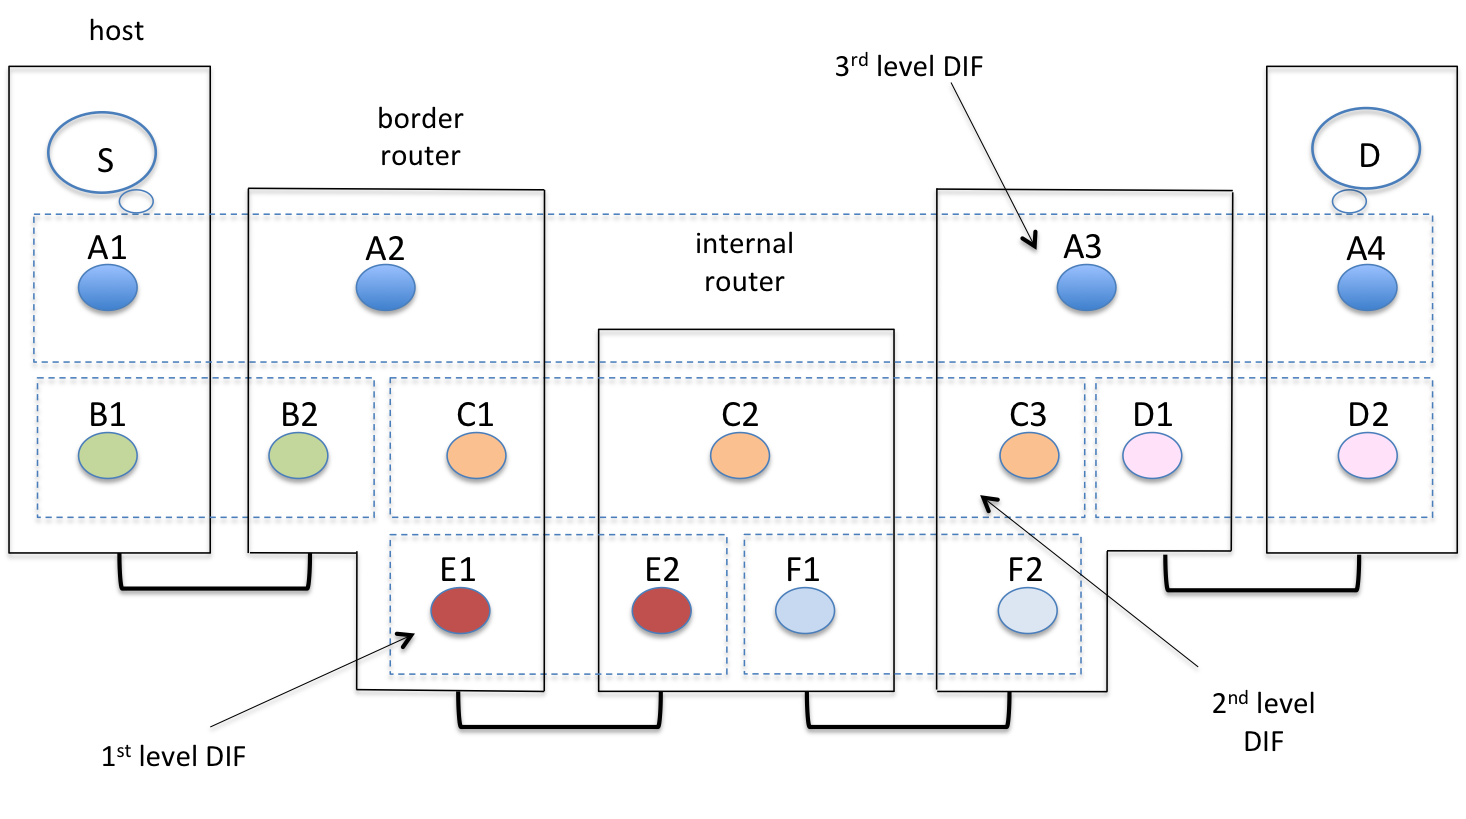
\includegraphics[width=\textwidth]{figures/rina-architecture}
    \caption{Recursive InterNetworking Architecture example \citep{website:irati}} 
    \label{fig:RINAexample}
\end{figure}
\npar
An example how communication between two processes would be established with RINA can be seen in the image~\ref{fig:RINAexample} above. Here we see application S on the host trying to communicate with application D on the other side of the communication chain. We see that for this specific example 3 levels of DIFs are used. These DIFs stack recursively from the bottom level (1st level) up till the DIF that actually takes care of the communication between the IPC and the application process. 


\section{IRATI implementation}
In this section we will address the technical implementation of the RINA model. The project that we will be using is the IRATI project. More information on this project can be found in the research question~\ref{sec:research_question}. 
\\
Here we opt to examine how the model is formed, what functions are already developed and which parts are useable yet. Finally we will quickly skim over the functions that are required for successfully finding an answer to our research question. 
\npar
The IRATI project is trying to build a working, open source, technical implementation of the Recursive InterNetworking Architecture \citep{website:irati_obj}. It focuses on tree main pillars: 

\begin{enumerate}
	\item Produce a working DIF over Ethernet 
	\item Provide an alternative to the current internet that delivers the same services
	\item Tackle current problem-cases of internet with the RINA alternative
\end{enumerate}

These goals engulf the entire project and can be seen as the coarse lines of the IRATI project. To complete all these goals we need to have several more specific subparts, one of these is the recently developed \textbf{RINA over Ethernet on UNIX-like Operation Systems}. This is one of the main goals of the project and almost all future work will use this as a foundation to build upon. Here a fully functional RIN\footnote{Recursive InterNetwork} architecture is being set up for Linux (UNIX-like) operating systems. After this is completed and other groundwork has been completed in the IRATI project it is finally the goal to open source this part of the project. This should provide a working Ethernet between UNIX-like OS's and open the road for applications to use RINA if they wish to do so after the release of the source code. 
\npar
A second component for the IRATI project is the Shim-DIF to handle TCP/IP traffic. Assuming that RINA will not be used as an island structure, meaning that RINA will still interact with the current implementation of the Internet. More specifically, RINA will still interact with TCP/IP traffic. To handle this traffic an adaptor DIF needs to be build. This adaptor DIF will be henceforth known as the TCP/IP Shim-DIF, since in the current IRATI project the amount of Shim-DIFs are limited to 1, we can shorten this to \textbf{Shim-DIF}. Consider a network where node A is on the current implementation of Internet, using TCP/IP and said node wants to communicate with node B also using this Internet with TCP/IP. Under normal conditions this would all be handled by TCP/IP interconnected nodes in between point A and B. However, hypothesize that some of these nodes in between A and B are running on RINA. This is where the need for a Shim-DIF is needed to encapsulate this TCP/IP stream, transfer the wrapped data using RINA towards the end-node of the the RINA network and unwrap it at that point. This means that when possible the data would be transferred with the RIN architecture, but this system would be flexible enough to handle the currently used TCP/IP protocol. Another example is when applications are not prepared yet for the switch to RINA and thus still use TCP/IP to set up communication. The top DIF, the one with direct interaction with the application, could wrap this data and become a Shim-DIF to help facilitate the communication the application is trying to set up. 
\npar
Once these goals have been acquired the expansion of the project can commence. This development can come from different angles. For example other operating systems could be tackled so the project can be run across multiple operating systems. Hereby we must state that the current goal is only to incorporate open source systems. The IRATI project is thinking about expanding towards the RIN architecture on JunOS, a FreeBSD-based operating system used in \emph{Juniper Networks \citep{website:junos}} routers. Here we can imagine a future where an entire network comprising of JunOS-based routers and workstations with UNIX-like OS's. Both fully equipped with RINA thanks to the IRATI project. This could lead to proper, full scale network testing and no longer pingpong tests between two nodes. 
\npar
Another expansion on the project could be made towards other protocols. In the transport layer we see that TCP\footnote{Transmission Control Protocol} is the most used one, but we also see that other protocols such as: 
\begin{quote}
\begin{description}
	\item[UDP] User Datagram Protocol
	\item[DCCP] Datagram Congestion Control Protocol
	\item[SCTP] Stream Control Transmission Protocol
	\item[RSVP] Resource Reservation Protocol
	\item[\ldots] \hfill
\end{description}
\end{quote}
In this project it has been decided to focus entirely on the TCP/IP protocol. However the goal of the project is to make the architecture so broad that it can work in function with other projects that focus on other protocols and even function in other operating scopes. This component is a co-developed part that should work alongside the Pouzin Society RINA project \citep{website:pouzin_society}. While PSOC\footnote{Pouzin SOCiety} focuses on UDP/IP in the middleware scope, IRATI aims towards TCP/IP in the kernel. When successful however this should not lead to any communication problems as both will be using the RINA prototype as a base system and thus they should be able to communicate. 
\npar
Of course are other groups and projects interested in RINA as it should provide an internet architecture that is clear, clean and works on a very basic principle. One of these projects is the OFELIA\footnote{OpenFlow in Europe: Linking Infrastructure and Applications}, this is an European project that provides researchers with a controllable test network. This project is especially interesting for IRATI because it provide a great testbed when not enough hosts, routers, switches, \ldots work on RINA. The working with the OFELIA project also works in the other direction. IRATI provides information towards OFELIA about the architecture. This allows the OFELIA project to expand and provide an adequate testbed for IRATI.
\npar
Finally we would like to briefly touch on where the thesis will fit in this project. The thesis is focused on the TCP/IP protocol on a UNIX-like Operating System. More specifically the thesis will aim to implement the IRATI stack on the Android platform, limited to TCP/IP. We see here that Android operating system counts as a UNIX-like operating system as Android is based on Linux, which in its own turn is a UNIX-like OS. The thesis will also focus on how to implement the TCP/IP Shim-DIF on wireless internet (802.11).


\section{Android restrictions}
While Android is a UNIX-like operating system and based on Linux, it does come with some restrictions. In this section we will be comparing Android OS to the Linux OS. The reason for this is that the IRATI project already has a working RINA implementation on Linux and this will be used for the further work of this thesis. Secondly because Android is based on Linux operating system and its kernel. At one point in history the two operating systems shared a common kernel and while this common component is planned, it is currently not the same kernel. 
\npar
Before we can further inspect the Android operating system, compared to Linux OS, we first need to identify the differences between the \textbf{Android kernel} and \textbf{Linux kernel}. For most of this information we will be using a talk by John Stultz, comparing Android to a stock Linux kernel \citep{presentation:android_linux_kernel,website:android_linux_kernel}. The amount of changes is not that large as it comprises of around 25 000 lines of changes, compared to the entire 15 millions lines of code for the full kernel. This places the changes around \textasciitilde0.2\% of the total code. Of course some of these changes can have large impacts on the actual kernel itself. These changes will be discussed here. Some of the items in the Android patches include:
\begin{itemize}
	\item Ashmem
	\item Binder
	\item Pmem
	\item Logger
	\item Early suspend
	\item Wakelocks
	\item Various small \emph{hacks} to facilitate a mobile OS
	\item \ldots
\end{itemize}
Because a Linux kernel is meant for desktop and server hardware (both very similar), Android aims to improve in the hardware department. This allows the use of more and varied hardware through its kernel. A second large point of interest for Android is the power management. While traditional systems are just plugged in with the cable and thus don't need to worry as much about power. The opposite is true for mobile, battery powered devices where power management is of utmost importance. Another change between the two kernels is the way error reporting is done and the attempt to increase security on the Android kernel. Finally the Android kernel aims to improve performance, especially for its intended users, mobile platforms.
\\
Some of these changes to the original kernel have been talked about quite a bit, such as the wakelocks. However we find that these changes should not impact the current implementation of the IRATI stack into Android. Further down the road additional optimization could be acquired between the Android kernel and the IRATI stack. An example here could be Binder, which is an IPC on its own and should thus be compatible with RINA. Also RINA should be able to work with Paranoid Networking so that networking does not become blocked by this feature in Android kernels. 
\npar
As shown above, the current version (and future versions) of the Android kernel should not pose any problems for the IRATI stack. However, an operating system does not only comprise of its kernel. This is an important part and the aspect where we see the biggest change between Linux and Android. When looking at a structured overview of an operating system (UNIX-like), we see that libraries play a big part in the undertaking of an operating system. Here we find the biggest change between Android and Linux. While Linux uses glibc \citep{website:glibc} and Android uses the Bionic library \citep{github:bionic,website:c_lib_bionic}. 
\npar
The restrictions from the Bionic library that affect the inclusion of the IRATI stack on Android are mostly limited to the \cpp language. The way Bionic handles \cpp is quite unique as it aims to alter the use of \cpp as a whole. This issue here is the following: IRATI stack is build on \cpp. For the most part \cpp is still supported by the library, but it does come with some restrictions. Before we inspect those restrictions we must first look at the reason why the glibc was not used in the first place. This can be declared very fast and accurate. Glibc is a \emph{slow} and \emph{huge} library. While this is not an issue for systems that run on Linux (desktops, servers, \ldots) it does form a problem for small-scale mobile platforms. Another issue with glibc is that it falls under GPL\footnote{GNU General Public License} and the smaller version, uClibC falls under LGPL\footnote{Lesser GNU General Public License}. This implies that everything that uses these libraries also falls under these licenses, something Google was looking to avoid. Hence the option to use a new library, Bionic, which uses as BSD license and thus can shield its applications from the GPL and LGPL licenses. Finally we must note that glibc is quite large and meant for high frequency processors, where bionic is a lot smaller and works very fast, even without high speed processors\footnote{High frequency CPUs are becoming available for mobile platforms at this very moment}.
\npar
Because the \cpp restrictions of the Bionic library are of utmost importance to this IRATI project inclusion we will now take a closer look at these restrictions. The most profound and important restriction is the lack of support for \cpp exceptions. Google engineers deemed these exceptions bloated and largely impractical for use thus the support for this was entirely cut. When people still want to use exceptions they are advised to try another library, add a library that does support these or switch to Java programming language in the userspace. This is an important change as the current IRATI project does use \cpp exceptions and thus the code will need to be retailored to fit seamless on the Android platform. Another option is to try and implement changes on Android so that the current IRATI project can be ported over. Secondly, Bionic does not contain a \cpp Standard Template Library. This is for obvious reasons to try and keep Bionic as small as possible. When applications wish to use a \cpp STL they will have to include one with the application or acquire it beforehand. Other changes bionic made can be viewed at Pthreads. These are threads that are standardized and should be compatible cross-platform. Some changes bionic made to these threads include: cancellation, pthread\_once(), pthread\_atfork(). Here it is recommended that when these functions are used in the original code, to revise the code and work around these changes. The changes are in place again to reduce the bloated code in glibc and endorse optimized coding. The final changes that bionic implements are the lack of support for wide and locale characters and some user-account-related functions. 
\npar
Finally we see that the biggest restrictions on Android come from the use of the Bionic library. This library limits some uses of \cpp and requires a bypass from the original application. We note that the IRATI project is written partially in \cpp and uses exceptions. This will require a workaround on either the operating system side or on the IRATI project. How this will be handled is one of the major questions in this thesis. 

\chapter{RINA on Android}


\section{Shim-DIF for wireless}
\section{WiFi Media Access Control}


\chapter{Conclusion and placement of the study in the thesis}

\section{Conclusion literature study}
\section{Placement of the literature study in the master thesis}

